\documentclass[11pt]{article}
\usepackage{amsmath,amssymb}
\usepackage{natbib}
\usepackage[hmargin=2cm,vmargin=4cm]{geometry}
\usepackage{color}
\usepackage{graphicx,wrapfig,lipsum}
\usepackage{hyperref}
\usepackage{titling}

\setlength{\droptitle}{-11em}   % This is your set screw

\title{Energy Disaggregation using Non-Intrusive Load Monitoring}

\author{Karen Yu, Nick Vasios and Thibaut Perol\\ \small Final project for AM207}
\date{}
\begin{document}
\maketitle


\section{Convolutional Neural Network (ConvNet)}
The implementation of the method presented in this section can be found in the notebook \url{https://github.com/tperol/am207-NILM-project/blob/master/Report_convnet.ipynb}. However the main codes are available in a separate repository (\url{https://github.com/tperol/neuralnilm}) to keep this final repository clean. Most of the codes for preprocessing of the data are borrowed from Jack Kelly repository that was forked (\url{https://github.com/JackKelly/neuralnilm}). However the implementation of the python generator for the data augmentation on CPU, the ConvNet implementation (trained on GPU) and post processing for the metrics are our own implementation.

\subsection{ConvNet introduction}
Convolutional Neural Networks are similar to ordinary Neural Networks (multi-layer perceptrons). Each neuron receive an input, perform a dot product with its weights and follow this with a non-linearity (here we only use ReLu activation functions). The whole network has a loss function that is here the Root Mean Square (RMS) error (details later). The network implements the 'rectangle method'. From the input sequence we invert for the start time, the end time and the average power of only one appliance (see Figure~\ref{convnet_architecture}).

\begin{figure}
\begin{center}
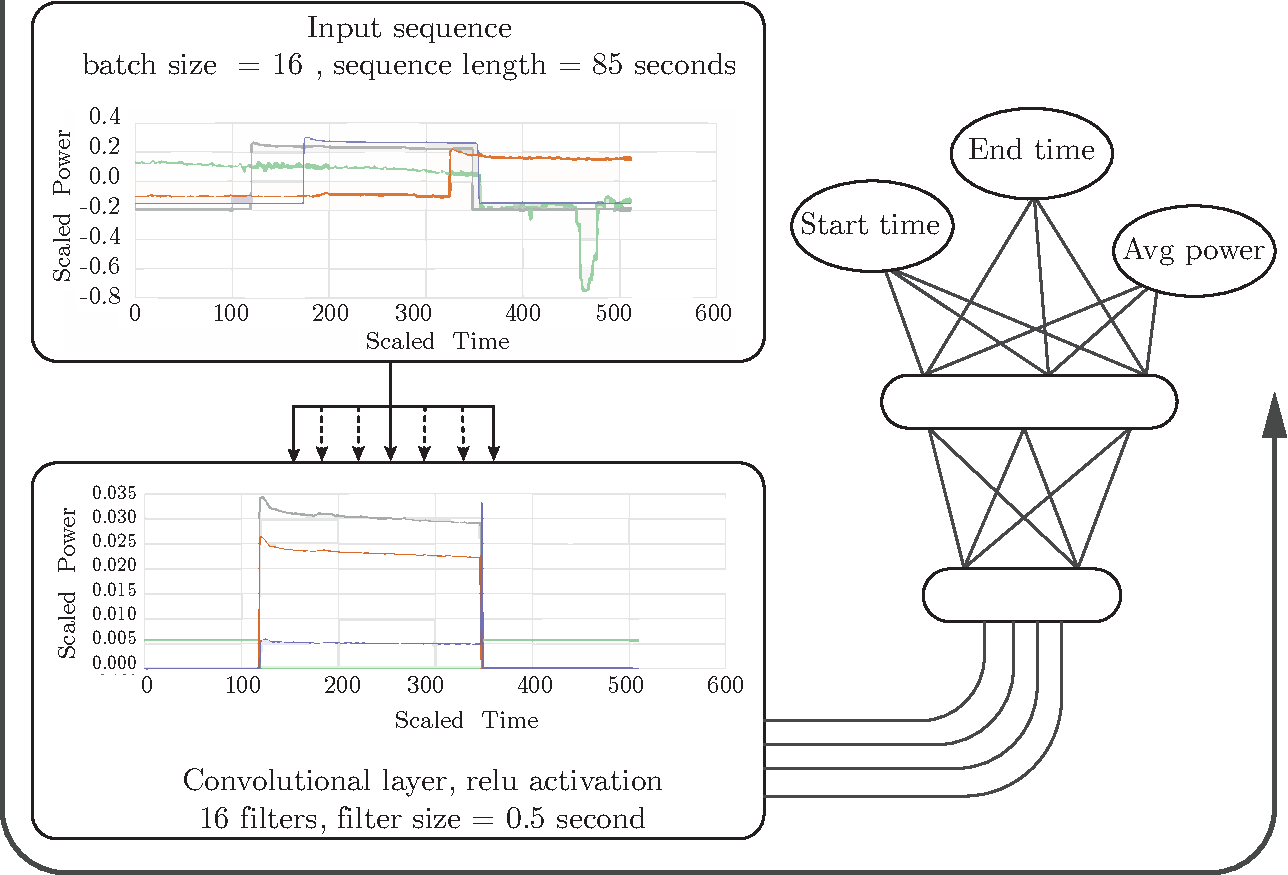
\includegraphics[width=29 pc]{./../poster/Figures/convnet_architecture}
\caption{A schematic representation of the architecture of the convolutional neural network}
\label{convnet_architecture}
\end{center}
\end{figure}

Convolutional neural networks have revolutionized computer vision. From an image the convolutional layer learns through its weights low level features. In the case of an image the features detectors (filters) would be: horizontal lines, blobs etc. These filters are built using a small receptive field and share weights across the entire input, which makes them translation invariant. Similarly, in the case of time series, the filters extract low level feature in the time series. By experimenting we found that only using 16 of these filters gives a good predictive power to the ConvNet. This convolutional layer is then flatten and we use 2 hidden layers of 1024 and 512 neurons with ReLu activation function before the output layer of 3 neurons (start time, end time and average power).

\subsection{Data pipeline}

\subsubsection{Selecting appliances}

We train each neural network per appliance. This is different from the CO and FHMM methods. For this report we only try to invert for the activation of the fridge and the microwave in the aggregated data. This two appliances have very different activation signatures (see Figure !!!).

\subsubsection{Selecting time sequences}

We downsampled  the main meters and the submeters to 6 samples per seconds in order to have the aggregated and the submeter sequences properly aligned. We throw away any activation shorter than some threshold duration to avoid spurious spikes. For each sequence we use 512 samples (about 85 seconds of recording).

\subsubsection{Selecting houses}

We choose to train the algorithm on house 1,2,3 and 6 and test the data on house 5.

\subsubsection{Dealing with unbalanced data: selecting aggregated data windows}

We first extract using NILMTK libraries (\url{http://nilmtk.github.io}) the target appliance (fridge or microwave) activations in the time series. We concatenate the times series from house 1,2,3, and 6 for the training set and will test on house 5. We feed to our neural network algorithm (detailed later) balanced mini-batches of data sequences of aggregated data in which the fridge is activated and sequences in which it is not activated. This is a way to deal with unbalanced data -- there are more sequences where the fridge is not activated than sequences with the fridge activated. Most of the data pipeline used is borrowed from \url{https://github.com/JackKelly/neuralnilm}.

\subsubsection{Synthetic aggregated data}

We use the method from Jack Kelly to create synthetic data. Two vectors of the size of the window fed to the network are initialized: the input and the target. The input is create with the combination of activations of the five most active appliances in each house. There is a 50 $\%$ chance that the target appliance will appear in the sequence and a 25 $\%$ chance for each other `distractor' appliance. We ran neural networks with and without synthetic aggregated data. We found that synthetic data acts as a regularizer, it improves the scores on unseen house.

\subsubsection{Standardization of the input data (aggregated data)}

A typical step in the data pipeline of neural network is the standardization of data. For each sequences of 512 samples (= 85 seconds) we subtract the mean to center the sequence. Furthermore every input sequence is divided by the standard deviation of a random sample in the training set. In this case we cannot divide each sequence by its own standard deviation because it would delete information about the scale of the signal. An example of 4 input sequences is shown in Figure~\ref{convnet_architecture}. 

\subsubsection{Output data (start time, end time and average power)}

The output of the neural network is 3 neurons: start time, end time and average power. We rescale the time to the interval [0,1]. Therefore if the fridge starts in the middle of the input sequences the output of the first neuron is 0.5. If its stops after the end of the input window the output of the second neuron is set to 1. The third neuron is the average power during the activation period. Of course this is set to 0 when it is not activated during the input sequence. We also post process the data by setting any start time lower than 0 to 0 and end time higher than 1 to 1. We create a average power threshold set to 0.1 that indicates if the appliance was active or not (under the threshold the appliance is considered off, above it is considered on).

Here we show as an example the input data and the output calculated by a trained network. We compare this with the real appliance activation.

\subsection{Scores}

Because of the dimension of the ouput we choose classification score metrics. When the starting time and the ending time are both 0 we call this a negative. We also call negative if the power average is lower than threshold. Otherwise this is positive (the appliance is activated). We call TP true positive, TN true negative, FP false positive and FN false negative. The various metrics/scores used in this study are
\begin{eqnarray}
recall = \frac{TP}{TP + FN} \\
 precision = \frac{TP}{TP + FP} \\
 F1 = 2 * \frac{precision* recall}{precision + recall} \\
 accuracy = \frac{TP + TN}{P + N}
\end{eqnarray}


\subsection{Implementation strategy for real time data augmentation}
While the neural network runs an NVIDIA GeForce GT 750M (GPU) we maintain the CPU busy doing the data augmentation in real time (load aggregated data, create the synthetic data, preprocess the mini-batch to be fed to the neural network). For this we create a python generator that creates a queue of 50 mini-batch and feed them successively to the GPU for training.
The pipeline class can be found in neuralnilm.data.datapiline at \url{https://github.com/tperol/neuralnilm} and is partially reproduced here. We do the same to generate the validation and test set.

\subsection{ConvNet architecture}


We use a convolutional neural network (ConvNet) to take advantage of the translation invariance. We want the ConvNet to recognize target appliance activation anywhere in the sequence. For this project we have tried multiple architecture that are reported later on. These architecture all have a first convolutional layer of filter size 3 and stride 1. We have played with both the filter size and the number of output filters on the first layer. We have found that 16 filters is a reasonable number -- increasing the number of filters in the first layer did not improve significantly the scores.
The best neural network we found consist of
\begin{enumerate}
\item Input layer: one channel and lenght of 512 samples
\item 1D convolutional layer (filter size = 3, stride = 1 , number of filters = 16, activation function = relu, border mode = valid, weight initialization = normal distribution)
\item Fully connected layer (N = 1024, activation function = relu, weight initialization = normal distribution)
\item Fully connected layer (N = 512, activation function = relu, weight initialization = normal distribution)
\item Fully connected layer (N= 3, activation function = relu)
\end{enumerate}
The ouput has 3 neurons activated by a relu activation function since the output cannot be negative. We have tried other networks that are reported later in this notebook. However this is the layout of the best one we found.


\subsection{Loss function and optimizer}
\subsubsection{Loss function}
Since the output neurons spans the real axis there is no other choice than using a L$_2$ norm for the loss function (Root Mean Square error). This is (predicted start time - true start time)$^2$ + (predicted end time - true end time)$^2$ + (predicted average power - true average power)$^2$. The total loss function is the sum of the loss function for all the sample in a mini-batch.


\subsection{Optimizer} 

We have tried various optimizer to find the best one. We used a classical Stochastic Gradient Descent to update the weights where we feed one mini-batch chosen randomly to the neural network and then update each weight
\begin{equation}
	w_j = w_j - \eta \frac{\partial L}{\partial w_j}
\end{equation}
where $L$ is the loss function evaluated for the given mini-batch. The gradient of the loss function is calculated using the backpropagation algorithm (not detailed here for simplicity). At each epoch we decrease the learning rate $\eta$ to allow the algorithm to converge towards a local minimum.

We tried a variation of SGD by using the momentum method. This method has some physical interpretation where $\mu$ is the friction coefficient. In this case the weights are update using
\begin{equation}
	w_j = w_j + \mu v - \eta \frac{\partial L}{\partial w_j}
\end{equation}
where $v$ is the velocity. An other tested implementation is the Nesterov momentum in which, at a given position in the landscape of weight we look one step ahead with the momentum and then evaluate the gradient there to calculate the new value of the weight. A pseudo code for this method is provided in the notebook (\url{https://github.com/tperol/am207-NILM-project/blob/master/Report_convnet.ipynb}). We found by experimenting that the best optimizer is Adam (http://arxiv.org/pdf/1412.6980v8.pdf). A pseudo code for this optimizer is provided in the notebook.

\subsection{Training and Validation losses}
We trained on GPU the network detailed earlier. We also experimented a network with two convolutional layers (see notebook). However it did not improve significantly the results. The training and validation losses are shown in Figure~\ref{fig:trainloss}. We stop the network after 20 epochs but the network was still learning ! The training is approximately 1 hours long on a GPU.

\begin{figure}
\begin{center}
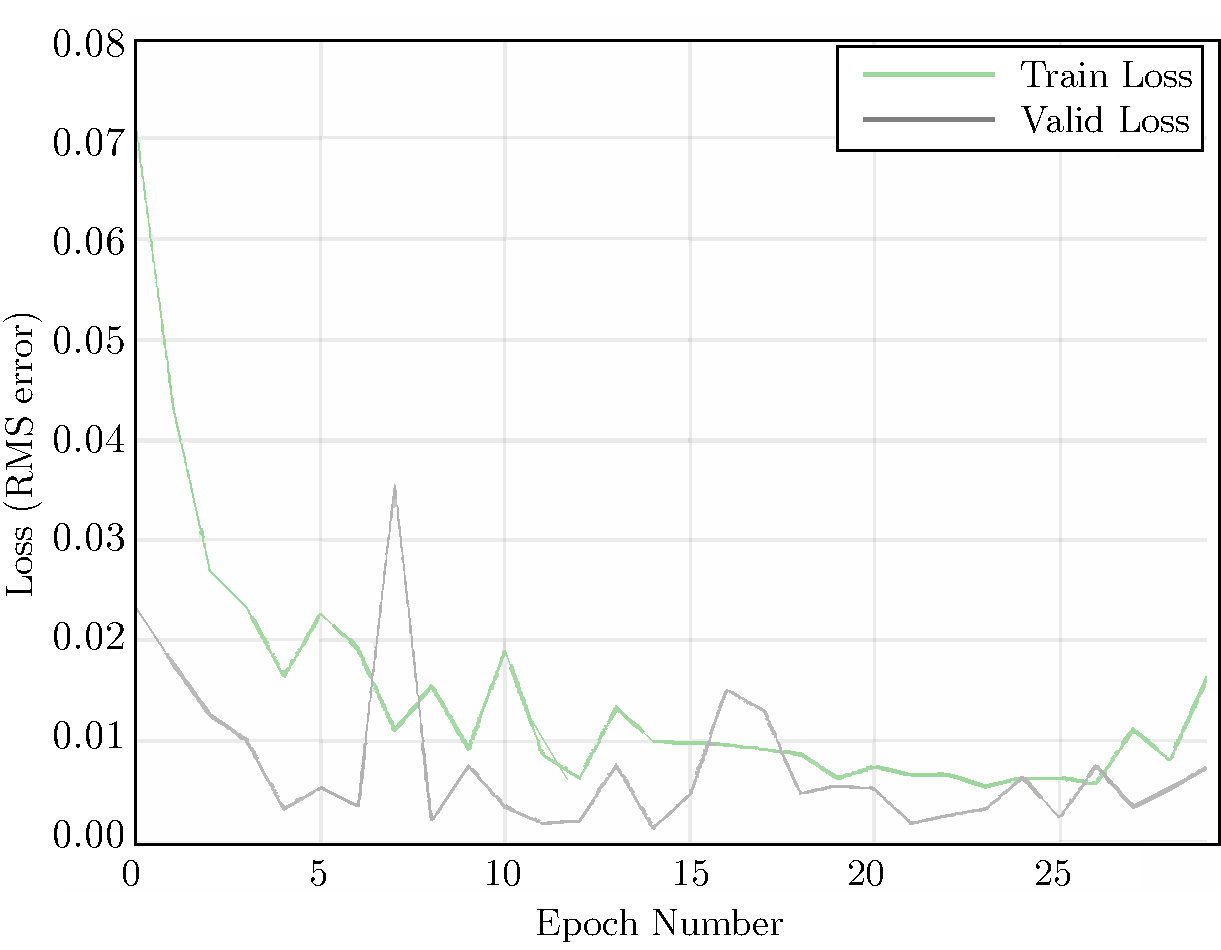
\includegraphics[width=20 pc]{./../poster/Figures/trainloss}
\caption{Training and validation loss during training of the ConvNet}
\label{fig:trainloss}
\end{center}
\end{figure}

\bibliographystyle{agufull08}
\bibliography{/Users/thibaut/Dropbox/Biblio/Perol_biblio}

\end{document}
